\section{Hệ cơ sở dữ liệu}
\subsection{Lí do sử dụng MongoDB}
MongoDB được lựa chọn vì nhiều ưu điểm:
\begin{itemize}
    \item \textit{Mô hình dữ liệu linh hoạt:} MongoDB cho phép mô hình hóa dữ liệu một cách tự nhiên và linh hoạt thông qua cấu trúc dữ liệu hướng tài liệu (document-oriented). Trong MongoDB, dữ liệu được lưu trữ dưới dạng các tài liệu JSON có cấu trúc linh hoạt, không yêu cầu định rõ cấu trúc trước đó như trong cơ sở dữ liệu quan hệ. Điều này cho phép chúng ta lưu trữ các thông tin đa dạng một cách tự nhiên. Mỗi tài liệu có thể chứa các trường khác nhau mà không cần phải tuân theo một lược đồ cố định, giúp dễ dàng thay đổi cấu trúc dữ liệu khi cần thiết. Ví dụ, hệ thống của nhóm cần lưu trữ các thông tin đa dạng về ngành nghề, thông tin cá nhân của người dùng, và các dữ liệu liên quan khác. Khi đó, việc MongoDB cho phép mô hình hóa dữ liệu một cách tự nhiên, linh hoạt, sẽ giúp chúng ta lưu trữ các thông tin này một cách hiệu quả và phản ánh đúng cấu trúc dữ liệu của ứng dụng.
    \item \textit{Khả năng mở rộng dễ dàng:} MongoDB cung cấp tính linh hoạt trong việc mở rộng bằng cách hỗ trợ cơ chế phân tán và scale-out. Với cơ chế phân mảnh (sharding), MongoDB cho phép phân tán dữ liệu trên nhiều máy chủ, giúp tăng khả năng chịu tải và lưu trữ dữ liệu lớn một cách hiệu quả. Ngoài ra, MongoDB cũng hỗ trợ các tính năng như replica sets để đảm bảo tính sẵn sàng và dự phòng, giúp hệ thống chịu lỗi tốt hơn. Trong trường hợp bước sang đồ án tốt nghiệp, nhóm muốn mở rộng tính năng IQ test, MongoDB có thể hỗ trợ bằng cách cho phép thêm các collection mới hoặc mở rộng các field trong collection hiện có một cách linh hoạt và dễ dàng.
    \item \textit{Truy vấn linh hoạt:} MongoDB cung cấp các tính năng truy vấn mạnh mẽ và linh hoạt như index, aggregation framework, và các câu lệnh truy vấn phong phú. Với index, MongoDB có thể tăng tốc độ truy xuất dữ liệu bằng cách tạo các chỉ mục trên các trường dữ liệu quan trọng. Aggregation framework cho phép thực hiện các phép tổng hợp, nhóm dữ liệu, và tính toán phức tạp trên các tài liệu trong một truy vấn duy nhất. Các câu lệnh truy vấn MongoDB linh hoạt và mạnh mẽ, hỗ trợ các phép toán như \$match, \$group, \$project để thực hiện các truy vấn phức tạp và đưa ra kết quả một cách hiệu quả.
\end{itemize}
\subsection{Cơ sở dữ liệu cho Ikigai Model}
\indent Hệ cơ sở dữ liệu được thiết kế cho Ikigai Model bao gồm 5 bảng như đã giới thiệu trong chương 3, phần 3.1. Phần này sẽ nói rõ cách hiện thực của nhóm trên cơ sở dữ liệu MongoDB
\indent Sau khi thu thập dữ liệu và tiến hành sử lí dữ liệu bằng pandas python sau đó chuyển những dữ liệu bao gồm các bảng chứa các document nhóm đã trình bày ở phần trên thành các file có định dạng  csv(comma-separated value) với mỗi hàng trong file là 1 document và 1 bảng là 1 file tương ứng. Sau đó nhập vào MongoDB từ chức năng "import csv" mà MongoDB cung cấp. \\
\indent Phần tiếp sau dây miêu tả trực tiếp mỗi bảng, vì mongoDB không yêu cầu kiểu dữ liệu, nhưng khi nhóm sử lí dữ liệu bằng pandas như đã nêu ở trên thì mỗi cột đều có kiểu dữ liệu riêng do đó ở phần này nhóm vẫn để kiểu dữ liệu vào trong phần giải thích để có cái nhìn tổng quan hơn về các documnet. \\
\newline
\indent Đối với dữ liệu của bài kiểm tra MBTI mỗi document bao gồm:
\begin{table}[H]
    \centering
    \begin{tabular}{@{}ll@{}}
        \toprule
        \textbf{Colums} & \textbf{Type} \\ \midrule
        MBTI & String \\
        Jobs & String \\ \bottomrule
    \end{tabular}
\end{table}

Đối với dữ liệu của bài kiểm tra Career Clustering mỗi document bao gồm:
\begin{table}[H]
    \centering
    \begin{tabular}{@{}ll@{}}
        \toprule
        \textbf{Colums} & \textbf{Type} \\ \midrule
        Career clustering & String \\
        Jobs & String \\ \bottomrule
    \end{tabular}
\end{table}

Với dữ liệu mức lương trung bình mỗi document bao gồm:

\begin{table}[H]
    \centering
    \begin{tabular}{@{}ll@{}}
        \toprule
        \textbf{Colums} & \textbf{Type} \\ \midrule
        Jobs & String \\
        Salary & int \\ \bottomrule
    \end{tabular}
\end{table}

Với dữ liệu nhu cầu nhân lực cho công việc mỗi document bao gồm:

\begin{table}[H]
    \centering
    \begin{tabular}{@{}ll@{}}
        \toprule
        \textbf{Colums} & \textbf{Type} \\ \midrule
        Jobs & String \\
        Jobs amount & int \\
        \bottomrule
    \end{tabular}
\end{table}

Dữ liệu gợi ý nghề nghiệp mỗi document bao gồm:
\begin{table}[H]
    \centering
    \begin{tabular}{@{}ll@{}}
        \toprule
        \textbf{Colums} & \textbf{Type} \\ \midrule
        Jobs & String \\
        Description & String \\
        Major & String \\
        \bottomrule
    \end{tabular}
\end{table}

Tổng hợp lại, ta có hệ cơ sở dữ liệu bao gồm:
\begin{figure}[H]
    \centering
    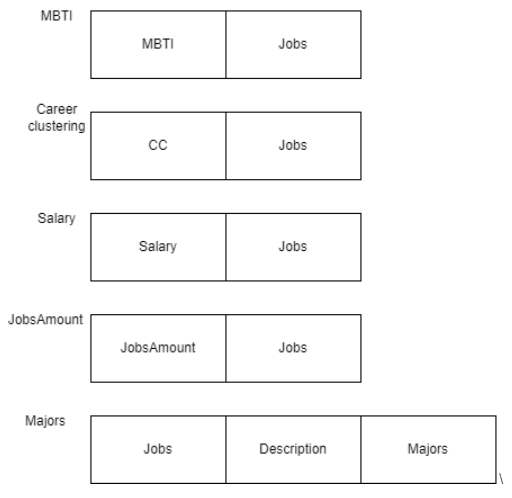
\includegraphics[width=0.6\linewidth]{images/database.png}
    \vspace{0.5cm}
    \caption{Hệ cơ sở dữ liệu}
\end{figure}

\subsection{Hệ cơ sở dữ liệu cho người dùng}
Hệ thống cũng hỗ trợ người dùng lưu trữ thông tin cá nhân và kết quả bài kiểm tra của họ. Dữ liệu người dùng được tổ chức thành các bảng sau:

\begin{figure}[H]
    \centering
    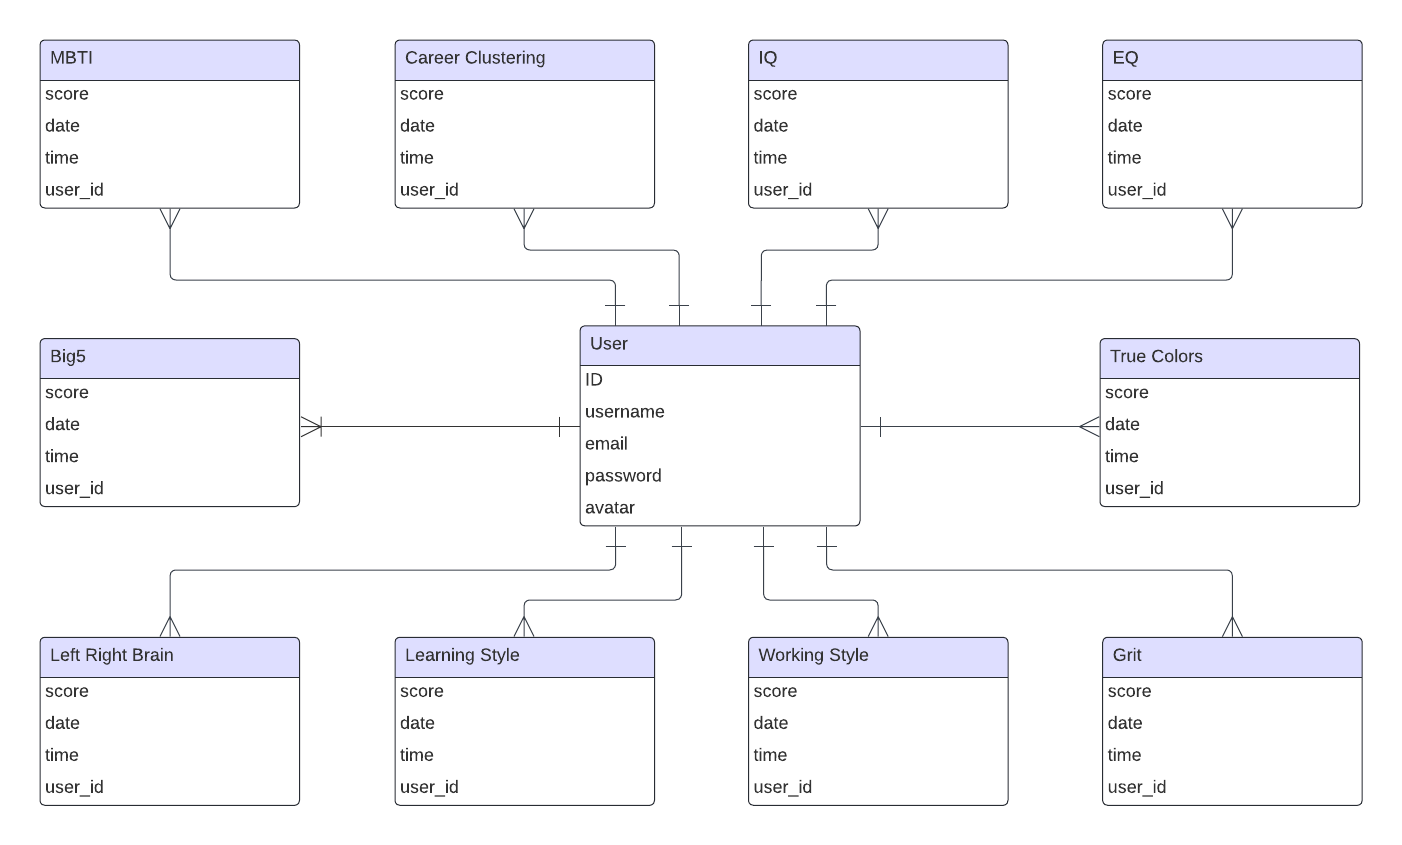
\includegraphics[width=1.0\linewidth]{images/usertable.png}
    \vspace{0.5cm}
    \caption{Hệ cơ sở dữ liệu}
\end{figure}

Mỗi bảng được tạo dưới dạng 1 collection trong MongoDB, với mỗi document trong collection là thông tin của một người dùng. Mỗi document bao gồm các trường thông tin như sau:
\begin{itemize}
    \item User: username, email, password, avatar, id
    \item Big5: score, date, time, user\_id
    \item Career cluster: score, date, time, user\_id
    \item Iq: score, date, time, user\_id
    \item Eq: score, date, time, user\_id
    \item Grit: score, date, time, user\_id
    \item Learning style: score, date, time, user\_id
    \item Mbti: score, date, time, user\_id
    \item Color: score, date, time, user\_id
    \item Left right brain: score, date, time, user\_id
    \item Working style: score, date, time, user\_id
\end{itemize}

Từ đó lưu trữ thông tin người dùng chung của họ, cũng như kết quả các bài kiểm tra cá nhân của họ để người dùng có thể dễ dàng xem lại cũng như
cải thiện bản thân mình.